\clearpage

\vspace{-0.25cm}
\section{Introduction}
\label{sec:introduction}

In this laboratory assignment, our aim was to design a band-pass filter (BPF)
with a central frequency, defined as the geometric mean of the lower and upper
cut-off frequencies, of 1 kHz and a gain at the central frequency of 40 dB.
For the design, the material available for use was as follows:

\begin{multicols}{2}
    \begin{itemize}
        \item One 741 OP-AMP
        \item At most three 1k$\Omega$ resistors
        \item At most three 10k$\Omega$ resistors
        \item At most three 100k$\Omega$ resistors
        \item At most three 220nF capacitors
        \item At most three 1$\mu$F capacitors
    \end{itemize}
\end{multicols}

With this in mind, the circuit we chose to use for this report was the following:
\begin{figure}[h] \centering
    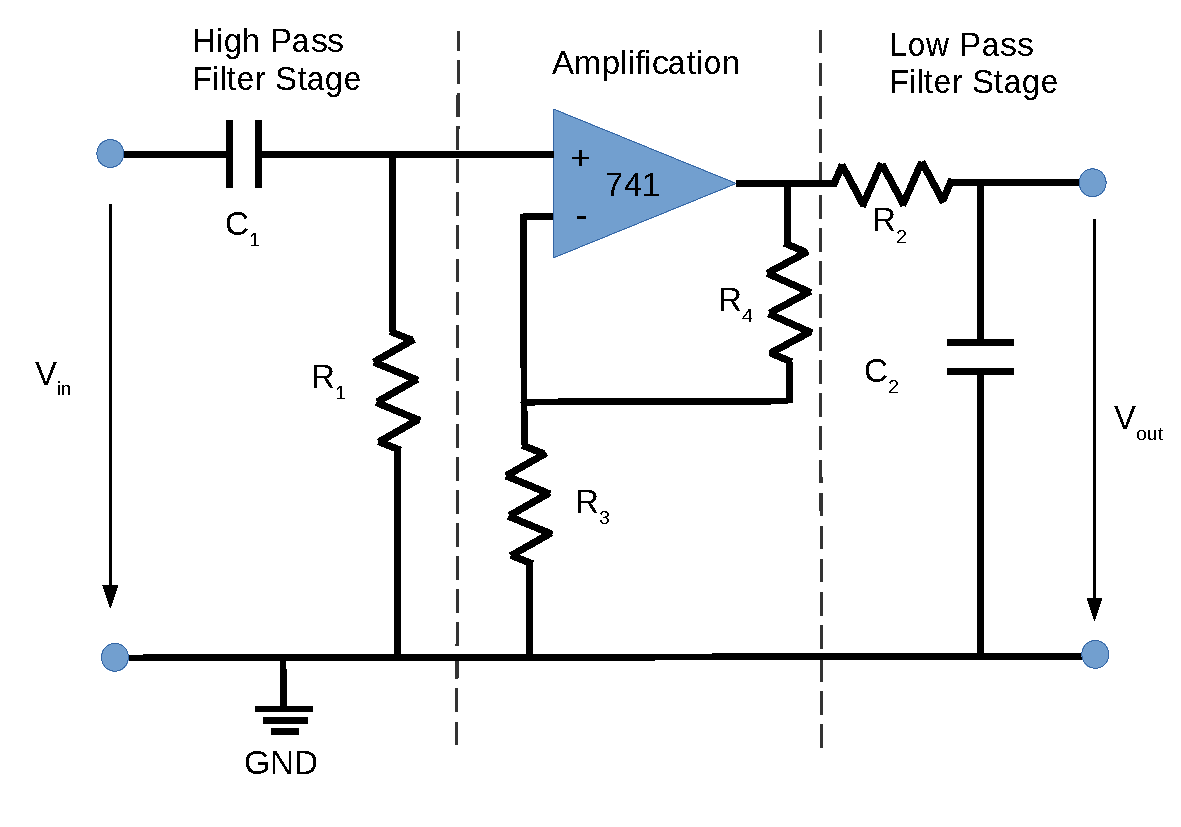
\includegraphics[scale=0.65]{lab5_principal.pdf}
    \caption{Band-pass filter circuit.}
    \label{fig:Principal}
\end{figure}


Basically the circuit consists of 3 stages: high pass filter, amplification and low pass filter in this exact order.
The first stage consists simply of a passive filter which attenuates low frequencies and lets through high frequency signals.
It is then followed by a non-inverting amplifier as shown.
Finally, to cut the highest frequencies, a passive RC filter was used,
which together with the previous high pass filter produces the desired
BPF.


In section \ref{sec:simulation}, using \emph{Ngspice}'s capabilities,
we improve the circuit by optimizing the values of
the resistors and capacitors and simulate the circuit in question.
Later, in section \ref{sec:analysis} we carry out a theoretical
analysis where we calculate the transfer function, input and output impedances
and the cut-off frequencies. Next we compare the results obtained
in both analyses and briefly discuss their possible similarities and differences in section \ref{sec:Comparison}.
Finally, in section \ref{sec:conclusion} we present our final thoughts regarding the work developed.